\documentclass{ximera}


\graphicspath{
  {./}
  {ximeraTutorial/}
  {basicPhilosophy/}
}

\newcommand{\mooculus}{\textsf{\textbf{MOOC}\textnormal{\textsf{ULUS}}}}

\usepackage{tkz-euclide}\usepackage{tikz}
\usepackage{tikz-cd}
\usetikzlibrary{arrows}
\tikzset{>=stealth,commutative diagrams/.cd,
  arrow style=tikz,diagrams={>=stealth}} %% cool arrow head
\tikzset{shorten <>/.style={ shorten >=#1, shorten <=#1 } } %% allows shorter vectors

\usetikzlibrary{backgrounds} %% for boxes around graphs
\usetikzlibrary{shapes,positioning}  %% Clouds and stars
\usetikzlibrary{matrix} %% for matrix
\usepgfplotslibrary{polar} %% for polar plots
\usepgfplotslibrary{fillbetween} %% to shade area between curves in TikZ
\usetkzobj{all}
\usepackage[makeroom]{cancel} %% for strike outs
%\usepackage{mathtools} %% for pretty underbrace % Breaks Ximera
%\usepackage{multicol}
\usepackage{pgffor} %% required for integral for loops



%% http://tex.stackexchange.com/questions/66490/drawing-a-tikz-arc-specifying-the-center
%% Draws beach ball
\tikzset{pics/carc/.style args={#1:#2:#3}{code={\draw[pic actions] (#1:#3) arc(#1:#2:#3);}}}



\usepackage{array}
\setlength{\extrarowheight}{+.1cm}
\newdimen\digitwidth
\settowidth\digitwidth{9}
\def\divrule#1#2{
\noalign{\moveright#1\digitwidth
\vbox{\hrule width#2\digitwidth}}}






\DeclareMathOperator{\arccot}{arccot}
\DeclareMathOperator{\arcsec}{arcsec}
\DeclareMathOperator{\arccsc}{arccsc}

















%%This is to help with formatting on future title pages.
\newenvironment{sectionOutcomes}{}{}


\title{Exponential Logarithmic}

\begin{document}

\begin{abstract}
percentage growth
\end{abstract}
\maketitle




The defining characteristic of linear functions is that the pairs experience a constant growth rate. If you calculate the rate of change between any two pairs, $(a, f(a))$ and $(b, f(b))$, in the function, you get the same value, $m$.


\[   \frac{f(b)-f(a)}{b-a} = m       \]

This led to the equation or formula for linear functions:  $f(x) = m(x-a) + f(a)$ \\





$\blacktriangleright$ Exponential functions are similar, but it is their \textbf{percentage} growth rate that is constant.   \\


\begin{example} Cancer Cells 

\link{https://www.ncbi.nlm.nih.gov/pmc/articles/PMC6695196/}

\textbf{Abstract:}. Most models of cancer cell population expansion assume exponential growth kinetics at low cell densities, with deviations to account for observed slowing of growth rate only at higher densities due to limited resources such as space and nutrients. [...] \\


\begin{image}
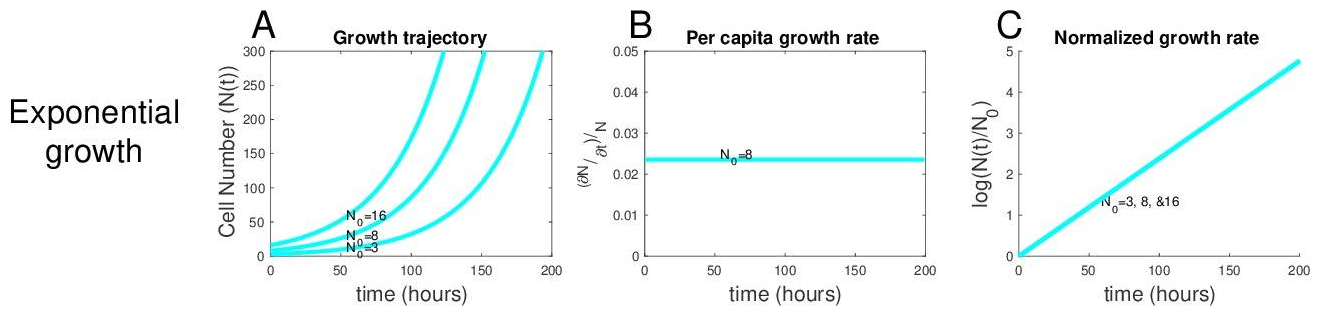
\includegraphics{pics/cancer_growth.png}
\end{image}


The number of cancer cells is given by $N(t) = N_0 \, e^{g \, t}$.

The graphs above show $N_0 = 3, 8, 16$

The first graph illustrate classical exponential growth.  \\

The second graph captures the "per capita growth rate".  This would be the growth in the number of cancer cells divided by the number of cancer cells. This gives the percentage growth.  The graph shows a constant function, because the percentage growth rate is a constant.

The third graph shows the logarithm of the first graph, which turns out to be a linear function.



\end{example}







The growth of an exponential function, $g(t)$ over the interval $[a, b]$ is $g(b)-g(a)$. To get a percentage, we compare this back to the starting value, $g(a)$: 

\[      \frac{g(b)-g(a)}{g(a)}    \]

And, then to get the percentage growth rate we average over the interval



\[      \frac{\frac{g(b)-g(a)}{g(a)}}{b-a}    \]



For an exponential function, this is constant


\[      \frac{\frac{g(b)-g(a)}{g(a)}}{b-a}  = r  \]

or

\[      \frac{g(b)-g(a)}{g(a)(b-a)}  = r  \]



Let's build such a function up from a given value of $g(0)$. 


\begin{procedure}
Moving from $0$ to $1$ gives

\[      \frac{\frac{g(1)-g(0)}{g(0)}}{1-0}  = r  \]


\[      g(1)-g(0) = r \, g(0)  \]


\[      g(1) = r \, g(0) + g(0)  \]

\[      g(1) =  g(0) (r + 1)  \]



Moving from $1$ to $2$ gives

\[      g(2) =  g(0) (r + 1)^2  \]


Moving from $2$ to $3$ gives

\[      g(3) =  g(0) (r + 1)^3  \]

\end{procedure}


In general, formulas for exponential functions look like


\[      g(t) = g(0) \cdot a^t   \]

















\section{Exponential Functions}


\begin{definition} \textbf{\textcolor{green!50!black}{Exponential Functions}}

Exponential functions are those functions that exhibit a constant percentage rate of change.  Their formulas look like


\[      f(x) = k \cdot a^x   \]

where $k$ is a nonzero real number, and $a$ is a positive real number.


\end{definition}


There are two types of exponential functions corresponding to $0<a<1$ or $1<a$.






\begin{itemize}
\item If $0<a<1$, then greater positive exponents make the function value smaller.   \\
In the other direction, a negative exponent essentially gives us the reciprocal of $a$, which would be greater than $1$ here.  Therefore, greater negative exponents result in bigger function values. \\

\item If $1<a$, then greater positive exponents make the function value bigger.   \\ 
In the other direction, a negative exponent essentially gives us the reciprocal of $a$, which would be less than $1$ here.  Therefore, greater negative exponents result in smaller postive function values.
\end{itemize}



The graphs of $y = Y(x) = 3 \cdot \left(\frac{1}{2}\right)^x$ and $z = W(t) = 3 \cdot 2^t$ are shown below.




\begin{image}
\begin{tikzpicture}
  \begin{axis}[name = leftgraph, 
            domain=-10:10, ymax=10, xmax=10, ymin=-10, xmin=-10,
            axis lines =center, xlabel=$x$, ylabel=$y$,
            every axis y label/.style={at=(current axis.above origin),anchor=south},
            every axis x label/.style={at=(current axis.right of origin),anchor=west},
            axis on top
          ]
          
          \addplot [line width=2, penColor, smooth, samples=200, domain=(-1.5:9),<->] {03*(0.5^x)};
   

  \end{axis}
  \begin{axis}[at={(leftgraph.outer east)},anchor=outer west, 
            domain=-10:10, ymax=10, xmax=10, ymin=-10, xmin=-10,
            axis lines =center, xlabel=$t$, ylabel=$z$,
            every axis y label/.style={at=(current axis.above origin),anchor=south},
            every axis x label/.style={at=(current axis.right of origin),anchor=west},
            axis on top
          ]
          
          \addplot [line width=2, penColor, smooth, samples=200, domain=(-9:2.1),<->] {2*(2^x)};


  \end{axis}



\end{tikzpicture}
\end{image}






There is no vertical asymptote.  The domain of exponential functions is all real numbers.  $y=0$ is a horizontal asymptote on both graphs. The sign of an exponential function is given by the coefficient.


Since these formulas are centered around the exponent, they follow the exponent rules:



\begin{itemize}
\item $a^n \cdot a^m = a^{n+m}$

\item $\frac{a^n}{a^m} = a^{n-m}$

\item $(a^n)^m = a^{n \cdot m}$

\item $a^n \cdot b^n = (a \cdot b)^n$

\item $\frac{a^n}{b^n} = \left(\frac{a}{b}\right)^n$


\end{itemize}




\begin{example}

Let $T(f) = 4 \cdot 3^f$.  Evaluate the following.

\begin{itemize}
\item $T(0) = \answer{4}$ 
\item $T(1) = \answer{12}$
\item $T(-1) = \answer{\frac{4}{3}}$
\end{itemize}
\end{example}























\section{Backwards}

What if we have a function value for an exponential function and we would like to know which domain numbers are associated with it.  In other words, we would like to solve


\[    g(t) = k \cdot a^t  =   g_0    \]


How would we solve for $t$?






\begin{example} If the function value "worked well", then we could probably guess.

Let $T(f) = 4 \cdot 3^f$.  


Solve $T(f) = 36$

$4 \cdot 3^f = 36$

$3^f = 9$

$f = 2$

\end{example}









Most function values are not going to be so obvious. 


For example, solve $ 3^x = 17$.


We may not be able to quickly think up this number or even an approximation for it.  However, we can still talk about.

\begin{center}
We are looking for the number that you raise $3$ to, to get $17$.
\end{center}


That is a specific number. We can see from the graph that there is only one such number and we could visually approximate it around $2.5$.


\begin{example}
The following are all descriptions that identify unique real numbers.

\begin{itemize}
\item The number that you raise $5$ to, to get $97$.
\item The number that you raise $\frac{3}{4}$ to, to get $6$.
\item The number that you raise $7$ to, to get $\frac{1}{2}$.
\item The number that you raise $101$ to, to get $34$.
\item The number that you raise $10$ to, to get $1,000$.
\end{itemize}

\end{example}



As with all mathematical phrases, we have shorthand notation for these desciptions.








\begin{definition} \textbf{\textcolor{green!50!black}{Logarithm Base A of B}}

Let $a$ and $b$ be positive real numbers.  The number  you raise $a$ to, to get $b$ is called the \textbf{logarithm base a of b}.

The symbol for the logarithm base a of b is $log_a(b)$.


$log_a(b)$ is  the number you raise $a$ to, to get $b$.

\[     a^{log_a(b)} = b          \]




\end{definition}





\begin{example}
The following are all descriptions that identify unique real numbers.

\begin{itemize}
\item The number that you raise $5$ to, to get $97$ is $log_5(97)$. \\
\item The number that you raise $\frac{3}{4}$ to, to get $6$ is $log_{\tfrac{3}{4}}(6)$. \\
\item The number that you raise $7$ to, to get $\frac{1}{2}$ is $log_7\left(\frac{1}{2}\right)$. \\
\item The number that you raise $101$ to, to get $34$ is $log_{101}(34)$. \\
\item The number that you raise $10$ to, to get $1,000$ is $log_{10}(1000)$. \\
\end{itemize}

\end{example}



\begin{example}
Evaluate the following expressions

\begin{itemize}
\item  $3^{log_3{56}} = \answer{56}$
\item  $13^{log_{13}{21}} = \answer{21}$
\item  $\pi^{log_{\pi}{82}} = \answer{82}$
\item  $4^{log_4{\sqrt{7}}} = \answer{\sqrt{7}}$
\item  $85^{log_{85}{2}} = \answer{2}$

\end{itemize}

\end{example}












Logarithms are exponents.  They can be positive or negative.



$9^{-2} = \frac{1}{81}$, therefore  $log_{9}\left(\frac{1}{81}\right) = -2$



We also know that raising a positve number to any exponent cannot produce a negative number or $0$.  Therefore, the number \textit{inside} the logarithm must be positive



It sounds like we have a new category of functions.




\begin{definition} \textbf{\textcolor{green!50!black}{Logarithmic Functions}}

A \textbf{Logarithmic Function} is a function that can be represented by formulas of the form

\[     L(x) =    log_a(x)            \]

where $a > 0$.

The domain is positive real numbers and the range is all real numbers.

\end{definition}








\begin{example}

Here is the graph of $y = L(x) = log_2(x)$.

\begin{image}
\begin{tikzpicture} 
  \begin{axis}[
            domain=-10:10, ymax=10, xmax=10, ymin=-10, xmin=-10,
            axis lines =center, xlabel=$x$, ylabel=$y$,
            ytick={-10,-8,-6,-4,-2,2,4,6,8,10},
            xtick={-10,-8,-6,-4,-2,2,4,6,8,10},
            ticklabel style={font=\scriptsize},
            every axis y label/.style={at=(current axis.above origin),anchor=south},
            every axis x label/.style={at=(current axis.right of origin),anchor=west},
            axis on top
          ]
          
          \addplot [line width=2, penColor, smooth,samples=200,domain=(0:9),<->] {ln(x)/ln(2)};
          \addplot [line width=1, gray, dashed,domain=(-9:9),<->] ({0},{x});

           

  \end{axis}
\end{tikzpicture}
\end{image}


The intercept is $(1,0)$, because $log_2(1) = 0$, because $2^0 = 1$.

On the interval $(0,1)$, we are looking at $log_2(x)$ for $0<x<1$.  Remember, $log_2(x)$ is the number you raise $2$ to, to get $x$, but here $0<x<1$.  Therefore, $2$ needs a negative exponent or $log_2(x) < 0$.  And, the smaller (closer to $0$) you want $x$, the bigger the negative exponent.





\end{example}



If we switch the base from something greater than $1$, to something less than $1$, then all of the exponents flip.  The graph flips.






\begin{example}

Here is the graph of $y = L(x) = log_{\tfrac{1}{2}}(x)$.

\begin{image}
\begin{tikzpicture} 
  \begin{axis}[
            domain=-10:10, ymax=10, xmax=10, ymin=-10, xmin=-10,
            axis lines =center, xlabel=$x$, ylabel=$y$,
            ytick={-10,-8,-6,-4,-2,2,4,6,8,10},
            xtick={-10,-8,-6,-4,-2,2,4,6,8,10},
            ticklabel style={font=\scriptsize},
            every axis y label/.style={at=(current axis.above origin),anchor=south},
            every axis x label/.style={at=(current axis.right of origin),anchor=west},
            axis on top
          ]
          
          \addplot [line width=2, penColor, smooth,samples=200,domain=(0:9),<->] {ln(x)/ln(0.5)};
          \addplot [line width=1, gray, dashed,domain=(-9:9),<->] ({0},{x});

           

  \end{axis}
\end{tikzpicture}
\end{image}


The intercept is $(1,0)$, because $log_{\tfrac{1}{2}}(1) = 0$, because $\left(\frac{1}{2}\right)^0 = 1$.

On the interval $(0,1)$, we are looking at $log_{\tfrac{1}{2}}(x)$ for $0<x<1$.  Now we just need large positive exponents of $\frac{1}{2}$ to get small numbers.  On the other hand, to get large positive numbers we need to raise $\frac{1}{2}$ to negative powers.





\end{example}







\end{document}
